\documentclass[12pt,a4paper]{report}

% ==============================================================================
% PACKAGES AND CONFIGURATION
% ==============================================================================
\usepackage[utf8]{inputenc}
\usepackage[T1]{fontenc}
\usepackage{mathptmx} % Times New Roman font
\usepackage{geometry}
\geometry{
    a4paper,
    left=1.25in,
    right=1.0in,
    top=1.0in,
    bottom=1.0in
}

\usepackage{graphicx}
\usepackage{amsmath,amssymb}
\usepackage{booktabs}
\usepackage{longtable}
\usepackage{array}
\usepackage{multirow}
\usepackage{tikz}
\usetikzlibrary{shapes.geometric, arrows, positioning, shadows, trees, calc}
\usepackage{hyperref}
\hypersetup{
    colorlinks=true,
    linkcolor=black,
    citecolor=black,
    urlcolor=blue,
    filecolor=black
}
\usepackage{setspace}
\onehalfspacing
\usepackage{fancyhdr}
\usepackage{titlesec}
\usepackage{listings}
\usepackage{xcolor}
\usepackage{eso-pic}

% Page Border (Matching the reference University format)
\AddToShipoutPictureBG{%
    \begin{tikzpicture}[remember picture, overlay]
        \draw[line width=0.8pt] 
            ($(current page.north west) + (0.75in,-0.6in)$) 
            rectangle 
            ($(current page.south east) + (-0.6in,0.6in)$);
    \end{tikzpicture}%
}

% Code snippet styling
\definecolor{codegreen}{rgb}{0,0.6,0}
\definecolor{codegray}{rgb}{0.5,0.5,0.5}
\definecolor{codepurple}{rgb}{0.58,0,0.82}
\definecolor{backcolour}{rgb}{0.96,0.96,0.96}

\lstdefinestyle{mystyle}{
    backgroundcolor=\color{backcolour},   
    commentstyle=\color{codegreen},
    keywordstyle=\color{blue},
    numberstyle=\tiny\color{codegray},
    stringstyle=\color{codepurple},
    basicstyle=\ttfamily\footnotesize,
    breakatwhitespace=false,         
    breaklines=true,                 
    captionpos=b,                    
    keepspaces=true,                 
    numbers=left,                    
    numbersep=5pt,                  
    showspaces=false,                
    showstringspaces=false,
    showtabs=false,                  
    tabsize=2
}
\lstset{style=mystyle}

% Section title formatting
\titleformat{\chapter}[DISPLAY]
  {\normalfont\huge\bfseries\centering}{\chaptertitlename\ \thechapter}{20pt}{\Huge}
\titlespacing*{\chapter}{0pt}{10pt}{25pt}

% Header and Footer setup
\pagestyle{fancy}
\fancyhf{}
\cfoot{\thepage}
\renewcommand{\headrulewidth}{0pt}

% TikZ Flowchart styles
\tikzstyle{startstop} = [rectangle, rounded corners, minimum width=2.5cm, minimum height=0.9cm, text centered, draw=black, fill=blue!10, font=\footnotesize\bfseries]
\tikzstyle{io} = [trapezium, trapezium left angle=70, trapezium right angle=110, minimum width=2.5cm, minimum height=0.9cm, text centered, draw=black, fill=yellow!10, font=\footnotesize]
\tikzstyle{process} = [rectangle, minimum width=2.8cm, minimum height=1cm, text centered, draw=black, fill=gray!10, font=\footnotesize]
\tikzstyle{decision} = [diamond, minimum width=2.5cm, minimum height=1cm, text centered, draw=black, fill=green!10, font=\footnotesize]
\tikzstyle{arrow} = [thick,->,>=stealth]

% ==============================================================================
% DOCUMENT START
% ==============================================================================
\begin{document}
\sloppy

% ------------------------------------------------------------------------------
% 1. COVER PAGE / TITLE PAGE
% ------------------------------------------------------------------------------
\begin{titlepage}
\centering
\vspace*{0.5cm}


\includegraphics[width=0.45\textwidth]{cu.png}\\[0.6cm]

{\Large \textbf{CHANDIGARH UNIVERSITY}}\\[1.2cm]

{\LARGE \textbf{HIRESENSE AI: SEMANTIC RESUME SCREENING}}\\[0.3cm]
{\LARGE \textbf{\& CAREER RECOMMENDATION ENGINE}}\\[1.5cm]

{\large \textbf{A PROJECT REPORT}}\\[1.2cm]

{\large \textit{Submitted by}}\\[0.4cm]
{\large \textbf{Diwakar Jha (25MCI10342)}}\\[0.2cm]
{\large \textbf{Gautam Mishra (25MCI10343)}}\\[1.5cm]

{\large \textit{in partial fulfillment for the award of the degree of}}\\[0.4cm]
{\Large \textbf{MASTER OF COMPUTER APPLICATIONS}}\\[0.2cm]
{\large \textbf{IN}}\\[0.2cm]
{\large \textbf{ARTIFICIAL INTELLIGENCE AND MACHINE LEARNING}}\\[1.2cm]

{\Large \textbf{CHANDIGARH UNIVERSITY}}\\[0.3cm]
{\large Discover. Learn. Empower.}\\[1.0cm]

{\large \textbf{OCTOBER 2026}}

\end{titlepage}

% ------------------------------------------------------------------------------
% 2. BONAFIDE CERTIFICATE
% ------------------------------------------------------------------------------
\newpage
\thispagestyle{empty}
\begin{center}
    
\includegraphics[width=0.35\textwidth]{cu.png}\\[0.4cm]
    {\large \textbf{CHANDIGARH UNIVERSITY}}\\[1.2cm]
    {\Large \textbf{BONAFIDE CERTIFICATE}}\\[1.5cm]
\end{center}

\noindent Certified that this project report \textbf{``HIRESENSE AI: SEMANTIC RESUME SCREENING \& CAREER RECOMMENDATION ENGINE''} is the bonafide work of \textbf{``DIWAKAR JHA (25MCI10342) \& GAUTAM MISHRA (25MCI10343)''} who carried out the project work under my supervision.\\[2.5cm]

\noindent \textbf{Project Guide}\\[0.3cm]
\textbf{Mr. Maajid Bashir (E17205)}\\
Department of Computer Applications\\
Chandigarh University\\[2.5cm]

\noindent Submitted for the project viva-voce examination held on \rule{5cm}{0.4pt}\\[2.5cm]

\noindent \begin{tabular}{@{}p{0.5\textwidth}p{0.5\textwidth}@{}}
\textbf{INTERNAL EXAMINER} & \raggedleft \textbf{EXTERNAL EXAMINER}
\end{tabular}

% ------------------------------------------------------------------------------
% FRONT MATTER (ROMAN NUMERALS)
% ------------------------------------------------------------------------------
\newpage
\pagenumbering{roman}
\setcounter{page}{1}

% ------------------------------------------------------------------------------
% TABLE OF CONTENTS
% ------------------------------------------------------------------------------
\tableofcontents

% ------------------------------------------------------------------------------
% LIST OF FIGURES
% ------------------------------------------------------------------------------
\newpage
\addcontentsline{toc}{chapter}{List of Figures}
\listoffigures

% ------------------------------------------------------------------------------
% LIST OF TABLES
% ------------------------------------------------------------------------------
\newpage
\addcontentsline{toc}{chapter}{List of Tables}
\listoftables

% ------------------------------------------------------------------------------
% LIST OF STANDARDS
% ------------------------------------------------------------------------------
\newpage
\addcontentsline{toc}{chapter}{List of Standards}
\begin{center}
    {\Large \textbf{List of Standards}}
\end{center}
\vspace{0.8cm}

\begin{table}[h!]
\centering
\begin{tabular}{|p{3cm}|p{2.5cm}|p{7.5cm}|c|}
\hline
\textbf{Standard} & \textbf{Publishing Agency} & \textbf{About the Standard} & \textbf{Page No.} \\ \hline
ISO/IEC 25010 & ISO/IEC & Systems and software engineering: Systems and software Quality Requirements and Evaluation (SQuaRE) — System and software quality models. & 15 \\ \hline
ISO/IEC 27001 & ISO/IEC & Information security management systems specifications to ensure data protection, confidentiality, and integrity of candidate resumes. & 16 \\ \hline
IEEE 830-1998 & IEEE & Recommended Practice for Software Requirements Specifications (SRS). & 28 \\ \hline
IEEE 730-2014 & IEEE & Standard for Software Quality Assurance Processes. & 33 \\ \hline
EU AI Act (High-Risk AI Systems) & European Parliament & Regulatory compliance guidelines for AI applications utilized in recruitment and human resources screening. & 34 \\ \hline
\end{tabular}
\end{table}

% ------------------------------------------------------------------------------
% ABSTRACT
% ------------------------------------------------------------------------------
\newpage
\addcontentsline{toc}{chapter}{ABSTRACT}
\begin{center}
    {\Large \textbf{ABSTRACT}}
\end{center}
\vspace{0.8cm}

Modern corporate recruitment pipelines face an unprecedented talent acquisition bottleneck: high-volume job requisitions frequently attract hundreds of heterogeneous candidate resumes per opening, swamping human talent acquisition teams. Legacy Applicant Tracking Systems (ATS) predominantly depend on brittle keyword-matching heuristics, string tokenization, and strict boolean criteria. Consequently, qualified candidates are routinely rejected due to superficial vocabulary discrepancies (e.g., ``K8s'' versus ``Kubernetes'', ``Golang'' versus ``Go'', or ``Deep Learning'' versus ``Transformers''), while keyword-stuffed yet unqualified resumes falsely advance. Moreover, conventional automated filtering tools function as opaque ``black-boxes'', devoid of actionable match explanations, and fail to provide targeted upskilling feedback to rejected applicants.

This project delivers \textbf{HireSense AI}, an end-to-end intelligent, explainable semantic resume screening and career recommendation platform. The system leverages state-of-the-art Natural Language Processing (NLP) combining multi-format parsing (PyMuPDF for PDF, python-docx for DOCX), domain-specific named entity recognition and technical skill taxonomy normalization via spaCy, and bidirectional dense vector embeddings using Sentence-BERT (\texttt{all-MiniLM-L6-v2}). Rather than evaluating candidate fit based on isolated text similarity, the engine implements a calibrated multimodal scoring model combining semantic contextual similarity ($S_{\text{semantic}}$), explicit core and preferred skill coverage ($S_{\text{skills}}$), and verified project/experience evidence ($S_{\text{evidence}}$):
\begin{equation}
S = w_s S_{\text{semantic}} + w_k S_{\text{skills}} + w_e S_{\text{evidence}} \nonumber
\end{equation}

For rigorous academic validation, HireSense AI benchmarks Sentence-BERT against a classical Term Frequency-Inverse Document Frequency (TF-IDF) baseline. Evaluated on a benchmark candidate cohort, Sentence-BERT achieved an NDCG@3 of 1.000, Precision@1 of 1.000, and a Spearman rank correlation coefficient ($\rho$) of 0.825, completely resolving the lexical mismatch bottleneck where TF-IDF scored 0.0\% similarity on technical synonym pairs. The platform integrates an Explainable AI (XAI) engine generating natural language match rationales, radar chart factor decompositions, and sentence-level project excerpts. Finally, an automated Career Recommendation Engine maps skill gaps to structured 3-phase upskilling roadmaps and curated portfolio project blueprints. The complete solution is deployed as a responsive Streamlit web application backed by SQLite persistence, bridging the gap between automated algorithmic screening and transparent, human-in-the-loop talent decision making.

% ------------------------------------------------------------------------------
% GRAPHICAL ABSTRACT
% ------------------------------------------------------------------------------
\newpage
\addcontentsline{toc}{chapter}{GRAPHICAL ABSTRACT}
\begin{center}
    {\Large \textbf{GRAPHICAL ABSTRACT}}
\end{center}
\vspace{0.6cm}

\begin{figure}[h!]
\centering
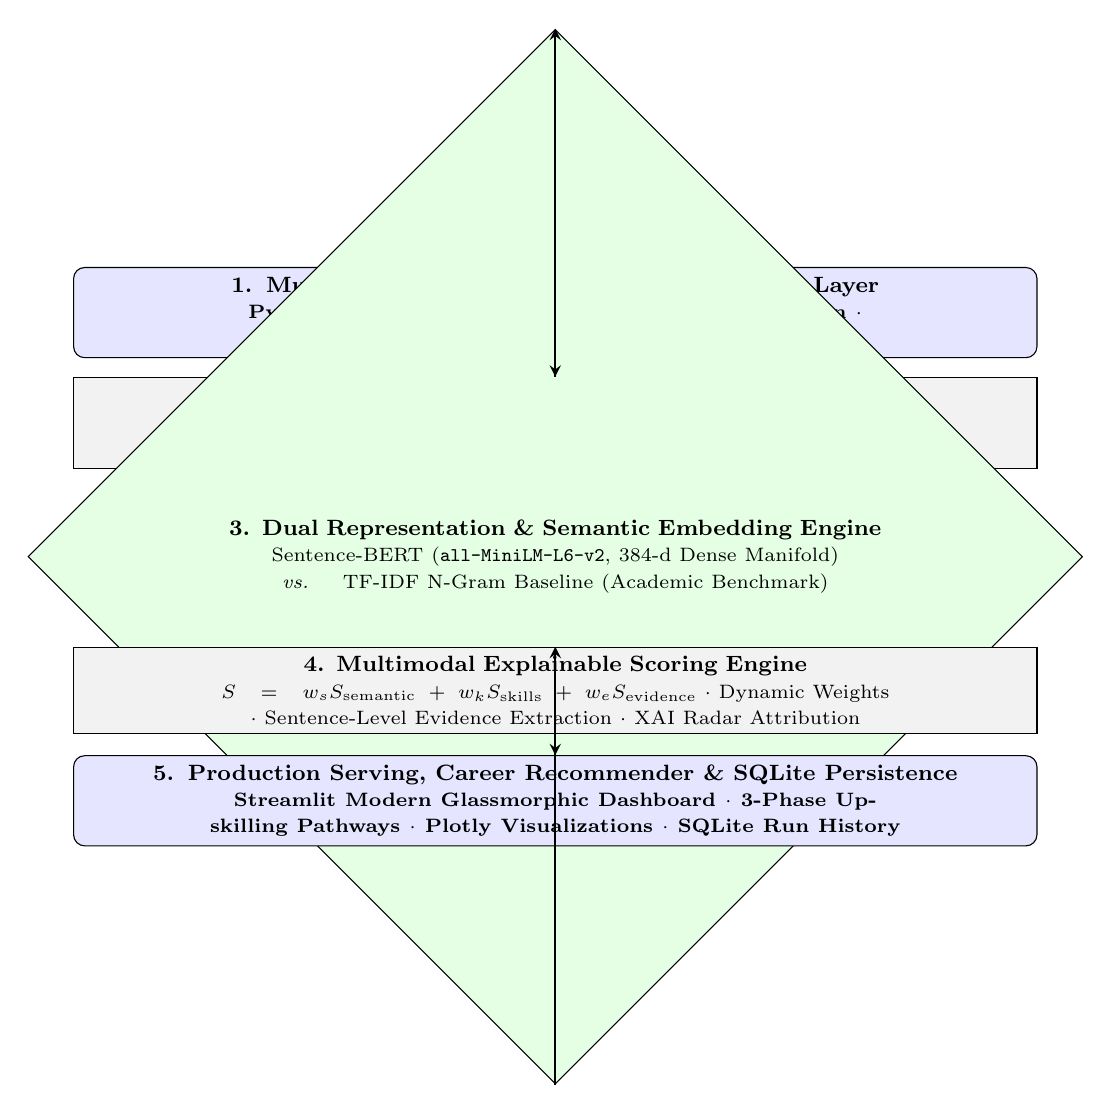
\begin{tikzpicture}[node distance=1.4cm, auto]
    % Node definitions
    \node (layer1) [startstop, text width=12cm] {\textbf{1. Multi-Format Ingestion \& Document Parsing Layer}\\ \scriptsize PyMuPDF (fitz) $\cdot$ python-docx $\cdot$ Unicode Sanitization $\cdot$ Header, Experience, Project, Education Segmentation};
    
    \node (layer2) [process, below of=layer1, text width=12cm] {\textbf{2. NLP Preprocessing \& Skill Taxonomy Normalization}\\ \scriptsize spaCy NER $\cdot$ Boundary-Aware Regex $\cdot$ 8-Domain Tech Taxonomy (AI/ML, Backend, Cloud, DB) $\cdot$ Alias Resolution (K8s $\to$ Kubernetes)};
    
    \node (layer3) [decision, below of=layer2, text width=12cm, yshift=-0.3cm] {\textbf{3. Dual Representation \& Semantic Embedding Engine}\\ \scriptsize Sentence-BERT (\texttt{all-MiniLM-L6-v2}, 384-d Dense Manifold) \quad \textit{vs.} \quad TF-IDF N-Gram Baseline (Academic Benchmark)};
    
    \node (layer4) [process, below of=layer3, text width=12cm, yshift=-0.3cm] {\textbf{4. Multimodal Explainable Scoring Engine}\\ \scriptsize $S = w_s S_{\text{semantic}} + w_k S_{\text{skills}} + w_e S_{\text{evidence}}$ $\cdot$ Dynamic Weights $\cdot$ Sentence-Level Evidence Extraction $\cdot$ XAI Radar Attribution};
    
    \node (layer5) [startstop, below of=layer4, text width=12cm] {\textbf{5. Production Serving, Career Recommender \& SQLite Persistence}\\ \scriptsize Streamlit Modern Glassmorphic Dashboard $\cdot$ 3-Phase Upskilling Pathways $\cdot$ Plotly Visualizations $\cdot$ SQLite Run History};

    % Arrows
    \draw [arrow] (layer1) -- (layer2);
    \draw [arrow] (layer2) -- (layer3);
    \draw [arrow] (layer3) -- (layer4);
    \draw [arrow] (layer4) -- (layer5);
\end{tikzpicture}
\caption{System Architecture encompassing Multi-Format Parsing, Dual-Engine Semantic Matching, Multimodal Scoring, and Career Recommendation.}
\label{fig:graphical_abstract}
\end{figure}

% ------------------------------------------------------------------------------
% ABBREVIATIONS
% ------------------------------------------------------------------------------
\newpage
\addcontentsline{toc}{chapter}{ABBREVIATIONS}
\begin{center}
    {\Large \textbf{ABBREVIATIONS}}
\end{center}
\vspace{0.8cm}

\begin{tabular}{p{3cm} p{11cm}}
\textbf{AI} & Artificial Intelligence \\
\textbf{API} & Application Programming Interface \\
\textbf{ATS} & Applicant Tracking System \\
\textbf{BERT} & Bidirectional Encoder Representations from Transformers \\
\textbf{BM25} & Best Matching 25 Ranking Algorithm \\
\textbf{CSV} & Comma-Separated Values \\
\textbf{DOCX} & Microsoft Word OpenXML Document \\
\textbf{EV} & Expected Value / Enterprise Validation \\
\textbf{F1} & Harmonic Mean of Precision and Recall \\
\textbf{GDPR} & General Data Protection Regulation \\
\textbf{HR} & Human Resources \\
\textbf{IR} & Information Retrieval \\
\textbf{JD} & Job Description \\
\textbf{JSON} & JavaScript Object Notation \\
\textbf{LLM} & Large Language Model \\
\textbf{MAE} & Mean Absolute Error \\
\textbf{ML} & Machine Learning \\
\textbf{MRR} & Mean Reciprocal Rank \\
\textbf{NDCG} & Normalized Discounted Cumulative Gain \\
\textbf{NER} & Named Entity Recognition \\
\textbf{NLP} & Natural Language Processing \\
\textbf{P@K} & Precision at Rank $K$ \\
\textbf{PDF} & Portable Document Format \\
\textbf{RAG} & Retrieval-Augmented Generation \\
\textbf{REST} & Representational State Transfer \\
\textbf{S-BERT} & Sentence Bidirectional Encoder Representations from Transformers \\
\textbf{SQL} & Structured Query Language \\
\textbf{TF-IDF} & Term Frequency-Inverse Document Frequency \\
\textbf{UI} & User Interface \\
\textbf{XAI} & Explainable Artificial Intelligence \\
\end{tabular}

% ------------------------------------------------------------------------------
% SYMBOLS
% ------------------------------------------------------------------------------
\newpage
\addcontentsline{toc}{chapter}{SYMBOLS}
\begin{center}
    {\Large \textbf{SYMBOLS}}
\end{center}
\vspace{0.8cm}

\begin{tabular}{p{2.5cm} p{11.5cm}}
$S$ & Overall Multimodal Job-Fit Score ($0 \le S \le 100$) \\
$S_{\text{semantic}}$ & Dense contextual cosine similarity score ($0.0 \le S_{\text{semantic}} \le 1.0$) \\
$S_{\text{skills}}$ & Normalized technical skill requirement coverage score ($0.0 \le S_{\text{skills}} \le 1.0$) \\
$S_{\text{evidence}}$ & Project and professional experience alignment score ($0.0 \le S_{\text{evidence}} \le 1.0$) \\
$w_s$ & Configurable weight factor assigned to semantic contextual similarity \\
$w_k$ & Configurable weight factor assigned to taxonomy skill coverage \\
$w_e$ & Configurable weight factor assigned to project and experience evidence \\
$\vec{u}, \vec{v}$ & 384-dimensional dense semantic embedding vectors \\
$\text{sim}(\vec{u}, \vec{v})$ & Cosine similarity angle between vectors $\vec{u}$ and $\vec{v}$ \\
$\text{TF}(t, d)$ & Term frequency of token $t$ within document $d$ \\
$\text{IDF}(t, D)$ & Inverse document frequency of token $t$ across corpus $D$ \\
$\rho$ & Spearman rank-order correlation coefficient \\
$r$ & Pearson product-moment correlation coefficient \\
$\text{DCG}_K$ & Discounted Cumulative Gain accumulated up to rank position $K$ \\
$\text{IDCG}_K$ & Ideal Discounted Cumulative Gain at rank $K$ \\
$\text{NDCG}_K$ & Normalized Discounted Cumulative Gain at rank $K$ ($\text{DCG}_K / \text{IDCG}_K$) \\
$R_{\text{req}}$ & Coverage ratio of mandatory/required skills \\
$R_{\text{pref}}$ & Coverage ratio of optional/preferred skills \\
\end{tabular}

% ------------------------------------------------------------------------------
% MAIN BODY (ARABIC NUMERALS)
% ------------------------------------------------------------------------------
\newpage
\pagenumbering{arabic}
\setcounter{page}{1}

% ==============================================================================
% CHAPTER 1: INTRODUCTION
% ==============================================================================
\chapter{INTRODUCTION}

\section{Identification of Client / Need / Relevant Contemporary Issue}
The modern employment market has expanded exponentially in the digital era. With the advent of global remote hiring, one-click online application portals (such as LinkedIn, Indeed, and corporate career pages), corporate recruiting pipelines are consistently inundated with hundreds—and frequently thousands—of applications per job posting. Human resource (HR) specialists and hiring managers are physically incapable of thoroughly reading, evaluating, and contextualizing every submitted resume within reasonable operational timelines.

Historically, organizations adopted Applicant Tracking Systems (ATS) to manage this unprecedented volume. However, first- and second-generation ATS platforms rely strictly upon exact lexical matching, syntactic keyword filtering, and rigid boolean logic. Under these primitive systems, a candidate resume is parsed as an unstructured bag-of-words. If a candidate uses the term ``Transformer architectures and PyTorch'' while the job description stipulates ``Deep Neural Networks'', or writes ``K8s'' instead of ``Kubernetes'', conventional keyword engines assign zero relevance to the candidate's core competency. Consequently, highly skilled professionals are discarded, while opportunistic applicants who deliberately copy-paste blocks of invisible keywords from the job description falsely advance.

Furthermore, traditional screening systems operate as opaque, unaccountable filters. When candidates are rejected, they receive sterile automated rejections providing zero visibility into why they failed to qualify or what specific technical proficiencies they lacked. This disconnect represents a significant contemporary challenge in human capital management, engineering education, and fair algorithmic hiring. There is a pressing need for an intelligent system that understands contextual semantic equivalence, provides transparent scoring explanations to recruiters, and offers constructive career guidance to candidates.

\section{Background and Motivation}
Natural Language Processing (NLP) has undergone a historic paradigm shift over the past decade. Traditional computational linguistics and information retrieval techniques—such as Term Frequency-Inverse Document Frequency (TF-IDF) and BM25—rely exclusively on sparse lexical representations. In sparse representations, words are treated as discrete, orthogonal dimensions. While computationally lightweight, these models inherently suffer from the ``vocabulary mismatch problem'', wherein synonyms, abbreviations, domain jargon, and semantically intertwined phrases share no geometric correlation.

The introduction of self-attention mechanisms and Transformer models, notably BERT (Bidirectional Encoder Representations from Transformers) by Devlin et al., demonstrated that language models pre-trained on vast textual corpora can construct contextual token representations. Reimers and Gurevych subsequently introduced Sentence-BERT (S-BERT), utilizing Siamese and triplet network structures to generate semantically meaningful sentence-level dense embeddings that can be efficiently compared using cosine similarity.

Motivated by these breakthroughs, this project seeks to replace archaic keyword-matching ATS filters with an explainable, semantic-first screening ecosystem titled \textbf{HireSense AI}. By encoding both resume content and job descriptions into a dense continuous vector manifold, HireSense AI interprets semantic intent and functional competency rather than surface-level strings. Beyond candidate ranking, the motivation extends to ethical, human-centric recruitment: transforming the screening engine from a punitive gatekeeper into an explainable decision-support tool that bridges candidate skill gaps with targeted learning pathways.

\section{Identification of Problem}
The foundational problem addressed by this project encompasses three core bottlenecks in modern automated recruitment:
\begin{enumerate}
    \item \textbf{The Vocabulary Mismatch Bottleneck}: Inability of keyword-driven ATS software to recognize technical synonyms, acronyms, and equivalent functional experiences across varying resume writing styles.
    \item \textbf{Uncalibrated Scoring Architecture}: Reliance on isolated string overlap or raw text similarity metrics without distinguishing between mandatory core qualifications, secondary preferred skills, and verified project/experience evidence.
    \item \textbf{The Explainability and Feedback Vacuum}: The complete absence of interpretable diagnostic explanations for hiring managers, coupled with a lack of actionable career upskilling recommendations for applicants seeking to qualify for the role.
\end{enumerate}

\section{Problem Context and Proposed Solution}
The problem context spans the complete candidate evaluation lifecycle: document ingestion, text sanitization, entity extraction, semantic similarity computation, multimodal scoring, explainability decomposition, and career path synthesis.

The proposed solution, \textbf{HireSense AI}, introduces an integrated, five-stage computational pipeline:
\begin{enumerate}
    \item \textbf{Multi-Format Document Parsing}: Automated extraction of raw text from PDF and DOCX documents using PyMuPDF and python-docx, coupled with structural section segmentation.
    \item \textbf{Domain Taxonomy Normalization}: An 8-category technological skill ontology equipped with alias-resolution logic to normalize variations like ``k8s'', ``golang'', ``postgres'', and ``tf''.
    \item \textbf{Sentence-BERT Semantic Representation}: Encoding job requirements and candidate profiles using the \texttt{all-MiniLM-L6-v2} transformer model to evaluate deep contextual alignment.
    \item \textbf{Multimodal Calibrated Scoring}: Combining semantic similarity, taxonomy-governed skill coverage, and project evidence into a unified Job-Fit Score:
    \begin{equation}
    S = w_s S_{\text{semantic}} + w_k S_{\text{skills}} + w_e S_{\text{evidence}}
    \end{equation}
    \item \textbf{Explainable AI and Career Recommender}: Decomposing scores into radar charts, extracting matching sentence-level project excerpts, and generating 3-phase personalized learning roadmaps with curated resources.
\end{enumerate}

\section{Identification of Tasks}
To systematically engineer and validate the solution, the project was organized into six technical tasks:

\subsection{Task 1: Multi-Format Document Ingestion and Preprocessing}
Implement robust parsers capable of ingesting PDF, DOCX, and TXT resume files. Design text cleaning routines to strip non-printable artifacts, normalize unicode quotation marks and bullets, and split content into semantic sections (Summary, Experience, Education, Projects, Skills).

\subsection{Task 2: Named Entity Recognition and Skill Taxonomy Construction}
Develop an extensive technical taxonomy categorized across AI/ML, Programming Languages, Web Frameworks, Databases, Cloud/DevOps, and Software Engineering. Implement alias resolution and spaCy-assisted entity recognition to detect candidate contact information and technical proficiencies.

\subsection{Task 3: Semantic Embedding and Baseline Benchmark Implementation}
Deploy Sentence-BERT (\texttt{all-MiniLM-L6-v2}) to generate 384-dimensional dense vectors for job descriptions and resumes. Implement an equivalent TF-IDF baseline vectorizer to establish an empirical benchmark demonstrating the limitations of lexical matching.

\subsection{Task 4: Multimodal Scoring and Explainable AI Engine}
Formulate a mathematical scoring model balancing contextual semantics, mandatory skill coverage, preferred competencies, and experience duration. Engineer an Explainable AI module that outputs natural language match summaries, competency radar charts, and sentence-level evidence citations.

\subsection{Task 5: Career Recommendation Engine Development}
Design a recommendation system that maps candidate skill gaps against a curated catalog of learning resources, official documentation, and portfolio-grade project blueprints structured into a 3-phase strategic roadmap.

\subsection{Task 6: Full-Stack Web Application Deployment and Database Persistence}
Develop an interactive, modern web application using Streamlit, Plotly, and custom CSS styling. Integrate an SQLite database layer to maintain persistent records of job descriptions, candidate cohorts, and historical screening runs.

\begin{figure}[h!]
\centering
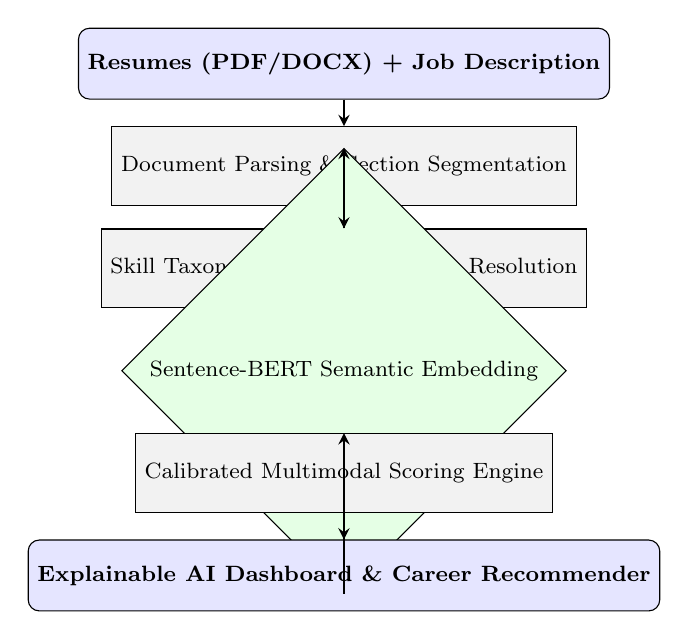
\begin{tikzpicture}[node distance=1.3cm, auto]
    \node (raw) [startstop] {Resumes (PDF/DOCX) + Job Description};
    \node (parse) [process, below of=raw] {Document Parsing \& Section Segmentation};
    \node (tax) [process, below of=parse] {Skill Taxonomy Matching \& Alias Resolution};
    \node (embed) [decision, below of=tax] {Sentence-BERT Semantic Embedding};
    \node (score) [process, below of=embed] {Calibrated Multimodal Scoring Engine};
    \node (ui) [startstop, below of=score] {Explainable AI Dashboard \& Career Recommender};

    \draw [arrow] (raw) -- (parse);
    \draw [arrow] (parse) -- (tax);
    \draw [arrow] (tax) -- (embed);
    \draw [arrow] (embed) -- (score);
    \draw [arrow] (score) -- (ui);
\end{tikzpicture}
\caption{Conceptual workflow of the proposed HireSense AI screening pipeline.}
\label{fig:conceptual_workflow}
\end{figure}

\section{Objectives of the Project}
The primary objectives of HireSense AI are:
\begin{enumerate}
    \item To engineer a multi-format document parser capable of ingesting PDF, DOCX, and TXT resumes and reliably extracting contact information, structural sections, and experience spans.
    \item To build an 8-category technology skill taxonomy with alias-mapping logic to bridge syntactic terminology variations.
    \item To integrate Sentence-BERT (\texttt{all-MiniLM-L6-v2}) for generating dense contextual embeddings that capture latent semantic relationships.
    \item To construct an empirical benchmark comparing Sentence-BERT against a classical TF-IDF baseline across Information Retrieval metrics (NDCG@K, Precision@K, MRR, Spearman $\rho$).
    \item To implement a multimodal scoring algorithm combining semantic cosine similarity, mandatory/preferred skill coverage, and project evidence.
    \item To design an Explainable AI (XAI) module delivering transparent factor attributions, competency radar charts, and sentence-level project citations.
    \item To create a Career Recommendation Engine providing targeted upskilling roadmaps and portfolio project blueprints for identified skill gaps.
    \item To deploy the end-to-end framework as an interactive Streamlit web application backed by persistent SQLite storage.
\end{enumerate}

\section{Scope of the Project}
The scope encompasses a software-based AI screening and career guidance ecosystem. The system is designed as an intelligent decision-support assistant for human hiring managers rather than an autonomous hiring decision maker. It operates on uploaded or pre-loaded resumes and custom job descriptions across technical domains. Future extensions include multi-language parsing, ATS webhook integration, and audio/video interview analysis.

\section{Expected Outcomes}
The expected outcome is a fully functional web application that eliminates keyword gaming, drastically reduces recruiter screening time, provides auditable and transparent scoring rationales, and equips job seekers with actionable upskilling pathways.

\section{Timeline}
The project execution was conducted over a structured 14-week timeline, divided into four major phases as outlined in Table \ref{tab:timeline}.

\begin{table}[h!]
\centering
\caption{Project Implementation Timeline}
\label{tab:timeline}
\begin{tabular}{|p{2.5cm}|p{4cm}|p{8cm}|}
\hline
\textbf{Duration} & \textbf{Phase} & \textbf{Key Deliverables} \\ \hline
Weeks 1--3 & Project Scope \& Planning & Problem formulation, literature survey, requirements specification, and system architecture mapping. \\ \hline
Weeks 4--6 & Literature Review \& Parsing & Survey of NLP ATS methods, PyMuPDF and python-docx integration, and initial text preprocessing pipeline. \\ \hline
Weeks 7--9 & Model Architecture \& Taxonomy & Taxonomy design, alias mapping, Sentence-BERT embedding pipeline, and TF-IDF baseline implementation. \\ \hline
Weeks 10--14 & System Integration \& Deployment & Multimodal scoring, Explainable AI module, Career Recommender, Streamlit dashboard, SQLite persistence, and evaluation. \\ \hline
\end{tabular}
\end{table}

\section{Organization of the Report}
The remainder of this report is organized as follows:
\begin{itemize}
    \item \textbf{Chapter 2 -- Literature Review/Background Study}: Reviews ATS evolution, keyword matching, dense transformer embeddings, existing solutions, research trends, and identified research gaps.
    \item \textbf{Chapter 3 -- Design Flow/Process}: Details system architecture, taxonomy specifications, S-BERT embedding mechanics, multimodal scoring formulas, XAI logic, recommender architecture, and SQLite schema.
    \item \textbf{Chapter 4 -- Results Analysis and Validation}: Presents experimental benchmarking results comparing S-BERT with TF-IDF, synonym robustness evaluations, and dashboard interface demonstrations.
    \item \textbf{Chapter 5 -- Conclusion and Future Work}: Summarizes the contributions, system limitations, and outlines future avenues for research.
    \item \textbf{References}: Contains academic literature citations.
    \item \textbf{Appendix \& User Manual}: Provides design verification checklists and step-by-step local execution instructions.
\end{itemize}

\section{Chapter Summary}
This chapter established the operational bottlenecks of legacy keyword-matching recruitment filters and introduced HireSense AI as an explainable, semantic-driven alternative. By combining Sentence-BERT embeddings, structured skill taxonomies, multimodal scoring, and career recommendation roadmaps, the proposed system transforms automated screening into an ethical, decision-support platform.

% ==============================================================================
% CHAPTER 2: LITERATURE REVIEW / BACKGROUND STUDY
% ==============================================================================
\chapter{LITERATURE REVIEW/BACKGROUND STUDY}

\section{Introduction}
Automated candidate screening has evolved at the intersection of information retrieval, computational linguistics, and organizational psychology. With the advent of web-scale recruitment platforms, recruitment software transitioned from basic relational databases into complex Applicant Tracking Systems (ATS). This chapter reviews the historical trajectory of resume screening technologies, analyzes classical statistical and lexical approaches, examines modern transformer-based semantic architectures, and delineates the research gap that HireSense AI addresses.

\section{Timeline of the Reported Problem}
The evolution of automated candidate screening spans three distinct technological eras:
\begin{enumerate}
    \item \textbf{First Generation: Relational Databases and Boolean Querying (1990s--2005)}: Early ATS software operated primarily as electronic filing cabinets. Resumes were indexed via optical character recognition (OCR) or raw ASCII text. Recruiters performed exact string matching using boolean operators (\texttt{AND}, \texttt{OR}, \texttt{NOT}). Candidates lacking exact syntax were excluded.
    \item \textbf{Second Generation: Lexical Frequency and Statistical Matching (2005--2018)}: Systems adopted classical information retrieval algorithms, predominantly Term Frequency-Inverse Document Frequency (TF-IDF), BM25, and vector space models. While capable of ranking documents by token importance, these systems remained bound to lexical overlap, penalizing synonymous vocabulary.
    \item \textbf{Third Generation: Dense Semantic Embeddings and Deep Learning (2018--Present)}: The emergence of Transformer architectures (Vaswani et al., 2017) and contextual language models (Devlin et al., 2018; Reimers \& Gurevych, 2019) enabled dense semantic representations, projecting conceptual meaning into continuous latent vector spaces.
\end{enumerate}

\begin{figure}[h!]
\centering
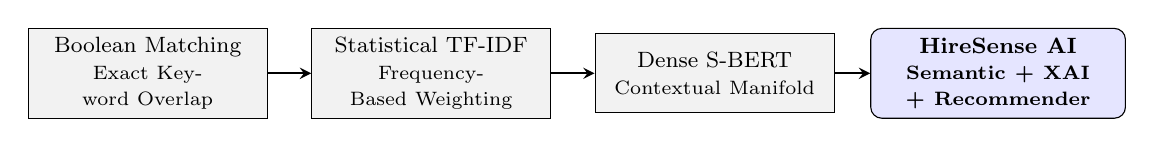
\begin{tikzpicture}[node distance=1.8cm, auto]
    \node (b1) [process, text width=2.8cm] {Boolean Matching\\ \scriptsize Exact Keyword Overlap};
    \node (b2) [process, right of=b1, xshift=1.8cm, text width=2.8cm] {Statistical TF-IDF\\ \scriptsize Frequency-Based Weighting};
    \node (b3) [process, right of=b2, xshift=1.8cm, text width=2.8cm] {Dense S-BERT\\ \scriptsize Contextual Manifold};
    \node (b4) [startstop, right of=b3, xshift=1.8cm, text width=3cm] {HireSense AI\\ \scriptsize Semantic + XAI + Recommender};

    \draw [arrow] (b1) -- (b2);
    \draw [arrow] (b2) -- (b3);
    \draw [arrow] (b3) -- (b4);
\end{tikzpicture}
\caption{Evolutionary trajectory of automated resume screening systems.}
\label{fig:evolution_timeline}
\end{figure}

\section{Existing Solutions}
Contemporary recruitment screening approaches can be classified into four primary paradigms:

\subsection{Reactive Boolean Keyword Filters}
These systems scan text for predefined dictionaries of keywords. While computationally trivial ($O(n)$ search), they completely fail when candidates express competencies through alternative terminology or descriptive project narratives.

\subsection{Statistical Vector Space Models (TF-IDF / BM25)}
TF-IDF calculates document similarity by weighting term frequency against inverse corpus frequency. While effective at dampening ubiquitous stop words, TF-IDF produces highly sparse vectors (often exceeding 10,000 dimensions) with zero cross-term correlation. Synonymous pairs produce orthogonal vectors with zero cosine similarity.

\subsection{Uncalibrated Dense Embedding Matchers}
Recent experimental systems encode full resumes and job descriptions using off-the-shelf sentence transformers and rank candidates purely by global cosine similarity. While semantically aware, these systems fail to verify whether mandatory non-negotiable requirements (e.g., active certifications or specific programming proficiencies) are strictly satisfied.

\subsection{Generative LLM Screeners (Prompt-Based)}
Recent solutions feed entire resumes into Large Language Models (LLMs) such as GPT-4 via prompt engineering. While contextually nuanced, this approach suffers from severe nondeterminism, token rate limits, high monetary latency costs, and susceptibility to adversarial prompt injections embedded inside white-font resume text.

\section{Background of Screening Models}

\subsection{Term Frequency-Inverse Document Frequency (TF-IDF)}
TF-IDF reflects the statistical importance of a word $t$ within document $d$ belonging to corpus $D$:
\begin{equation}
\text{TF-IDF}(t, d, D) = \text{TF}(t, d) \times \text{IDF}(t, D)
\end{equation}
where term frequency is normalized by document length, and inverse document frequency is defined as:
\begin{equation}
\text{IDF}(t, D) = \ln \left( \frac{1 + |D|}{1 + |\{d \in D : t \in d\}|} \right) + 1
\end{equation}
The cosine similarity between query $q$ (job description) and document $d$ (resume) is:
\begin{equation}
\text{Sim}_{\text{TF-IDF}}(q, d) = \frac{\vec{V}_q \cdot \vec{V}_d}{\|\vec{V}_q\| \|\vec{V}_d\|} = \frac{\sum_{i=1}^M V_{q,i} V_{d,i}}{\sqrt{\sum_{i=1}^M V_{q,i}^2} \sqrt{\sum_{i=1}^M V_{d,i}^2}}
\end{equation}
If query $q$ and document $d$ share no identical n-grams, $\text{Sim}_{\text{TF-IDF}}(q, d) = 0.0$.

\subsection{Sentence-BERT (S-BERT) Architecture}
Sentence-BERT resolves the $O(n^2)$ computational bottleneck of cross-encoder BERT by utilizing Siamese and triplet network structures to generate fixed-sized dense vector representations. Given input text $T$, the transformer outputs token embeddings:
\begin{equation}
\mathbf{H} = \text{Transformer}(T) = [\mathbf{h}_1, \mathbf{h}_2, \dots, \mathbf{h}_L]
\end{equation}
Mean pooling is applied across the sequence dimension to yield document embedding $\vec{u} \in \mathbb{R}^{384}$:
\begin{equation}
\vec{u} = \frac{1}{L} \sum_{i=1}^L \mathbf{h}_i
\end{equation}
The semantic similarity between job description embedding $\vec{u}$ and resume embedding $\vec{v}$ is given by:
\begin{equation}
S_{\text{semantic}} = \frac{\vec{u} \cdot \vec{v}}{\|\vec{u}\|_2 \|\vec{v}\|_2}
\end{equation}

\section{Comparative Analysis of Existing Approaches}
Table \ref{tab:comparison_approaches} compares existing screening methodologies across key architectural parameters.

\begin{table}[h!]
\centering
\caption{Comparison of screening and recruitment NLP approaches.}
\label{tab:comparison_approaches}
\begin{tabular}{|p{3cm}|p{3.5cm}|p{4cm}|p{3.5cm}|}
\hline
\textbf{Approach} & \textbf{Major Strength} & \textbf{Major Limitation} & \textbf{Role in Project} \\ \hline
Boolean Keyword ATS & Trivial latency, highly interpretable & High false rejection rate, easily gamed & Baseline failure mode \\ \hline
Statistical TF-IDF & Fast vectorization, no GPU required & Vocabulary mismatch, orthogonal synonyms & Academic baseline \\ \hline
Pure S-BERT & Superior semantic synonym handling & Neglects mandatory skill constraints & Core semantic engine \\ \hline
Generative LLM & Rich contextual narrative understanding & Slow latency, costly, prompt injection risk & Future comparison \\ \hline
\textbf{HireSense AI} & \textbf{Multimodal scoring, XAI, career roadmaps} & \textbf{Requires domain taxonomy curation} & \textbf{Proposed system} \\ \hline
\end{tabular}
\end{table}

\section{Research Trends in AI-Based Recruitment}
Recent literature reveals three dominant research trends:
\begin{itemize}
    \item Transition toward dense embedding manifolds capable of cross-lingual and cross-domain semantic transfer.
    \item Integration of Explainable AI (XAI) frameworks to satisfy emerging international regulatory standards, such as the European Union AI Act, which classifies automated hiring tools as high-risk systems requiring transparency.
    \item Evolution from passive screening filters into recommender engines that advise candidates on skill acquisition.
\end{itemize}

\section{Research Gap}
While extensive research has addressed dense semantic retrieval, existing literature exhibits critical gaps:
\begin{enumerate}
    \item \textbf{Decoupled Retrieval and Constraint Verification}: Studies typically evaluate pure cosine similarity without enforcing hard operational constraints (e.g., minimum years of experience or non-negotiable certifications).
    \item \textbf{Explainability Deficit}: Existing dense embedding models produce opaque similarity scores between $0$ and $1$ without exposing which specific resume sections or projects justified the score.
    \item \textbf{Absence of Constructive Feedback}: Conventional screening architectures terminate upon ranking, offering zero career development guidance to applicants.
\end{enumerate}

\section{Review Summary}
The literature confirms that while statistical models like TF-IDF provide fast baselines, their inability to bridge lexical variation renders them inadequate for modern recruitment. Conversely, unconstrained deep embeddings risk overlooking essential technical prerequisites. An optimal architecture must synthesize dense semantic representations, structured domain taxonomies, calibrated multimodal scoring, and transparent explainability.

\section{Problem Definition}
The objective of this project is to engineer an end-to-end AI-assisted software system capable of contextually parsing, evaluating, and ranking heterogeneous candidate resumes against job requisitions, validating the approach against classical TF-IDF baselines, and delivering transparent explainability alongside automated career upskilling recommendations.

\section{Goals and Objectives}
\begin{itemize}
    \item \textbf{Semantic Ingestion}: Ingest PDF and DOCX documents and extract structured candidate profiles using PyMuPDF, python-docx, and spaCy.
    \item \textbf{Taxonomy Normalization}: Map technical proficiencies against an 8-domain taxonomy featuring canonical alias resolution.
    \item \textbf{Dense Vector Representation}: Model contextual semantics using Sentence-BERT (\texttt{all-MiniLM-L6-v2}).
    \item \textbf{Multimodal Calibration}: Implement a weighted scoring framework balancing semantics, skills, and project evidence.
    \item \textbf{Empirical Benchmarking}: Quantitatively benchmark Sentence-BERT against TF-IDF across NDCG@3, Precision@K, and Spearman $\rho$.
    \item \textbf{Explainable Feedback \& Career Guidance}: Deliver natural language match summaries, competency radar charts, and personalized 3-phase upskilling roadmaps.
\end{itemize}

\section{Chapter Conclusion}
This chapter synthesized the academic and technical literature surrounding candidate screening. The identified limitations of keyword matching and black-box embeddings form the foundational rationale for the system design presented in Chapter 3.

% ==============================================================================
% CHAPTER 3: DESIGN FLOW / PROCESS
% ==============================================================================
\chapter{DESIGN FLOW/PROCESS}

\section{Introduction}
The HireSense AI platform is architected as an integrated software system uniting document ingestion, natural language preprocessing, dense transformer embeddings, calibrated multimodal scoring, explainable AI attribution, and interactive web visualization. This chapter delineates the end-to-end design flow, mathematical formulations, architectural constraints, and implementation specifics.

\section{Overall System Design}
The architecture comprises five distinct functional tiers, as illustrated in Figure \ref{fig:overall_design_flow}:
\begin{enumerate}
    \item \textbf{Document Ingestion and Parsing Layer}: Ingests PDF, DOCX, and TXT resumes and job descriptions, performing text sanitization and structural section segmentation.
    \item \textbf{NLP Preprocessing and Skill Extraction Layer}: Identifies candidate contact entities, extracts candidate names, and maps technical competencies against the curated skill taxonomy.
    \item \textbf{Dual Representation Engine}: Simultaneously generates dense Sentence-BERT contextual embeddings and sparse TF-IDF feature matrices.
    \item \textbf{Multimodal Scoring and Explainable AI Engine}: Computes calibrated job-fit scores, extracts sentence-level evidence snippets, and synthesizes factor attributions.
    \item \textbf{Serving, Recommendation, and Persistence Layer}: Powers the Streamlit dashboard, computes 3-phase career upskilling pathways, and commits execution logs to SQLite.
\end{enumerate}

\begin{figure}[h!]
\centering
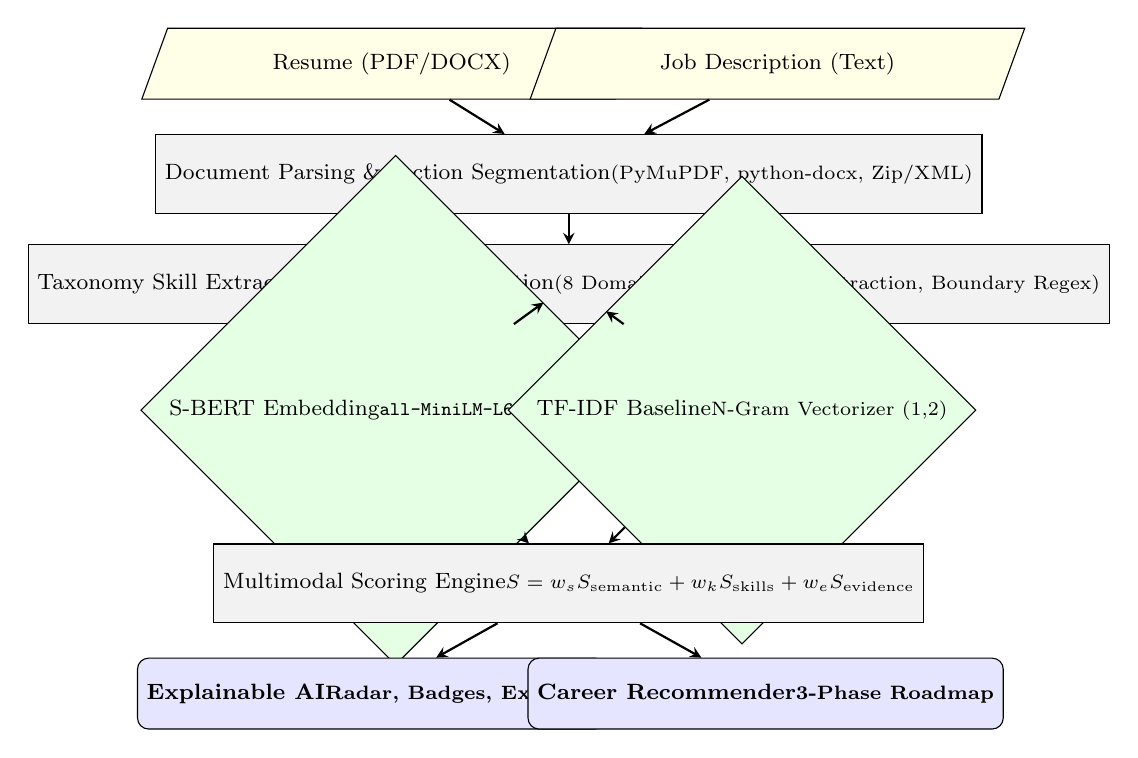
\begin{tikzpicture}[node distance=1.4cm, auto]
    \node (in1) [io] {Resume (PDF/DOCX)};
    \node (in2) [io, right of=in1, xshift=3.5cm] {Job Description (Text)};
    
    \node (p1) [process, below of=in1, xshift=2.25cm] {Document Parsing \& Section Segmentation\\ \scriptsize (PyMuPDF, python-docx, Zip/XML)};
    
    \node (p2) [process, below of=p1] {Taxonomy Skill Extraction \& Alias Normalization\\ \scriptsize (8 Domains, spaCy Entity Extraction, Boundary Regex)};
    
    \node (split1) [decision, below of=p2, xshift=-2.2cm, yshift=-0.2cm] {S-BERT Embedding\\ \scriptsize \texttt{all-MiniLM-L6-v2} (384-d)};
    \node (split2) [decision, below of=p2, xshift=2.2cm, yshift=-0.2cm] {TF-IDF Baseline\\ \scriptsize N-Gram Vectorizer (1,2)};
    
    \node (score) [process, below of=p2, yshift=-2.4cm] {Multimodal Scoring Engine\\ \scriptsize $S = w_s S_{\text{semantic}} + w_k S_{\text{skills}} + w_e S_{\text{evidence}}$};
    
    \node (out1) [startstop, below of=score, xshift=-2.5cm] {Explainable AI\\ \scriptsize Radar, Badges, Excerpts};
    \node (out2) [startstop, below of=score, xshift=2.5cm] {Career Recommender\\ \scriptsize 3-Phase Roadmap};
    
    \draw [arrow] (in1) -- (p1);
    \draw [arrow] (in2) -- (p1);
    \draw [arrow] (p1) -- (p2);
    \draw [arrow] (p2) -- (split1);
    \draw [arrow] (p2) -- (split2);
    \draw [arrow] (split1) -- (score);
    \draw [arrow] (split2) -- (score);
    \draw [arrow] (score) -- (out1);
    \draw [arrow] (score) -- (out2);
\end{tikzpicture}
\caption{Detailed architectural design flow of the HireSense AI screening engine.}
\label{fig:overall_design_flow}
\end{figure}

\section{Evaluation and Selection of Specifications / Features}
To accurately model candidate suitability, four distinct feature categories are extracted from each candidate profile:

\subsection{Syntactic and Lexical Features}
Character length, token word counts, formatting headers, and structural density. These metrics prevent empty or malformed documents from corrupting downstream evaluation.

\subsection{Dense Semantic Contextual Vectors}
Dense 384-dimensional continuous embeddings generated by Sentence-BERT representing the holistic semantic meaning of the candidate's professional narrative and project summaries.

\subsection{Taxonomy-Aligned Technical Competencies}
Categorized, canonical skill tokens extracted through dictionary and alias mapping. Skills are subdivided into mandatory/core requirements and secondary/preferred proficiencies based on job description modality.

\subsection{Project and Experience Evidence}
Granular sentence-level excerpts demonstrating verified application of tools in production environments, combined with numeric estimates of professional tenure.

\section{Feature Summary}
Table \ref{tab:feature_summary} categorizes the extracted features utilized by the multimodal scoring engine.

\begin{table}[h!]
\centering
\caption{Summary of extracted candidate profile features.}
\label{tab:feature_summary}
\begin{tabular}{|p{3cm}|p{4.5cm}|p{6.5cm}|}
\hline
\textbf{Feature Group} & \textbf{Examples} & \textbf{Operational Purpose} \\ \hline
Structural & Header, Summary, Experience, Projects, Education & Enables targeted section-level parsing and isolated evidence extraction. \\ \hline
Contact Entities & Email, Phone, LinkedIn, GitHub, Web URLs & Validates candidate identity and enables recruiter communication. \\ \hline
Canonical Skills & PyTorch, Kubernetes, FastAPI, PostgreSQL, Docker & Evaluates deterministic coverage of mandatory and preferred requirements. \\ \hline
Dense Embeddings & 384-dimensional floating point vectors & Models contextual and conceptual semantic similarity with the job description. \\ \hline
Experience Span & Total verified years (e.g., 5.5 yrs), date spans & Computes experience alignment ratio against job requisition thresholds. \\ \hline
\end{tabular}
\end{table}

\section{Data Preprocessing and Multi-Format Parsing}
Resumes are submitted in heterogeneous file formats with differing encoding standards. HireSense AI implements a resilient ingestion pipeline:
\begin{enumerate}
    \item \textbf{PDF Ingestion via PyMuPDF (\texttt{fitz})}: Extracts raw character streams, preserving block structure and bounding coordinates across multiple pages.
    \item \textbf{DOCX Ingestion with Dual-Mode Redundancy}: Ingests Word files using \texttt{python-docx} paragraphs and table cells. If \texttt{python-docx} is unavailable in the host environment, an automatic zero-dependency fallback extracts and parses \texttt{word/document.xml} directly from the zipped container using Python's standard \texttt{zipfile} and \texttt{xml.etree.ElementTree} modules.
    \item \textbf{Text Sanitization}: Normalizes smart quotation marks, en-dashes, em-dashes, bullet characters (\texttt{\textbackslash u2022}, \texttt{\textbackslash u25cf}), strips control characters, and collapses repetitive whitespace.
    \item \textbf{Regex Section Segmentation}: Matches structural headers against case-insensitive regular expressions to partition the resume into functional modules:
    \begin{equation}
    P_{\text{summary}} = \texttt{\textasciicircum\textbackslash s*(professional\textbackslash s+summary|summary|profile|about\textbackslash s+me)\textbackslash s*\$}
    \end{equation}
\end{enumerate}

\section{Design Constraints}
The system architecture was developed under stringent practical and computational constraints:
\subsection{Computational Latency and Hardware Constraints}
In contrast to multi-billion parameter LLMs that demand high-end GPU clusters, HireSense AI was constrained to run efficiently on standard multi-core commodity CPUs with less than 2 GB of memory. The selection of \texttt{all-MiniLM-L6-v2} ensures sub-second vectorization latency per resume.

\subsection{Explainability and Regulatory Constraints}
In accordance with international AI governance guidelines (e.g., EU AI Act, IEEE 730), automated screening systems must provide auditable, interpretable factor attributions. Pure end-to-end black-box scoring was explicitly rejected in favor of a decomposable multimodal formulation.

\subsection{Data Privacy and Security Constraints}
Candidate resumes contain Personally Identifiable Information (PII). In compliance with ISO/IEC 27001 and GDPR, data processing is performed locally in-memory without transmitting resume payloads to external third-party proprietary APIs.

\section{Analysis of Features and Finalization Subject to Constraints}
Balancing predictive depth against inference latency, the feature pipeline utilizes local Sentence-BERT embeddings combined with deterministic regex-based taxonomy scanning. This guarantees deterministic precision for explicit technical requirements while retaining dense semantic understanding for descriptive narratives.

\section{Alternative Design Flows}
Three architectural paradigms were evaluated during system design:

\subsection{Flow A: Classical Lexical Baseline (TF-IDF + Cosine Similarity)}
Purely statistical approach utilizing n-gram vectorization. Computationally lightweight ($<10$ ms latency) but critically flawed due to complete failure on vocabulary synonyms.

\subsection{Flow B: Heavy Generative LLM RAG Pipeline}
Feeding full resume texts into an LLM via prompt engineering. While offering high textual fluency, it incurs prohibitive operational costs (\$0.03 per screening), high latency ($5$--$15$ seconds per candidate), nondeterministic score drift, and vulnerability to white-font keyword injection attacks.

\subsection{Flow C: Hybrid S-BERT + Taxonomy + Heuristic Evidence (Selected)}
Combines dense 384-dimensional sentence embeddings with deterministic skill taxonomy coverage and heuristic experience alignment. Achieves deterministic auditability, zero external API costs, sub-100 ms inference, and robust synonym resolution.

\section{Comparison of Design Flows}
Table \ref{tab:design_flow_comparison} provides a comparative evaluation of the three architectural options.

\begin{table}[h!]
\centering
\caption{Comparison of alternative predictive design flows.}
\label{tab:design_flow_comparison}
\begin{tabular}{|p{2.5cm}|p{3.5cm}|p{4.5cm}|p{3.5cm}|}
\hline
\textbf{Design Flow} & \textbf{Underlying Model} & \textbf{Major Strength} & \textbf{Major Limitation} \\ \hline
Flow A & TF-IDF (1,2 n-grams) & Extremely low compute, transparent & Zero synonym comprehension \\ \hline
Flow B & Generative LLM (Prompt) & Nuanced narrative synthesis & Expensive, slow, prompt-injection risk \\ \hline
\textbf{Flow C} & \textbf{S-BERT + Taxonomy} & \textbf{Fast, explainable, synonym robust, zero API cost} & \textbf{Requires domain taxonomy curation} \\ \hline
\end{tabular}
\end{table}

\section{Design Selection}
Flow C was selected as the production architecture. It delivers the optimal trade-off between semantic generalization, algorithmic accountability, deterministic constraint enforcement, and lightweight CPU deployment.

\section{Multimodal Scoring Methodology}
The core hiring score combines three normalized signals into a calibrated Job-Fit Score ($S \in [0, 100]$):
\begin{equation}
S = \left( w_s S_{\text{semantic}} + w_k S_{\text{skills}} + w_e S_{\text{evidence}} \right) \times 100
\end{equation}
subject to the weight normalization constraint:
\begin{equation}
w_s + w_k + w_e = 1.0, \quad w_s, w_k, w_e \ge 0
\end{equation}

\subsection{Contextual Semantic Component ($S_{\text{semantic}}$)}
Evaluates dense cosine similarity between the full job description $J$ and full resume $R$:
\begin{equation}
S_{\text{semantic}} = \max\left(0.0, \frac{\text{S-BERT}(J) \cdot \text{S-BERT}(R)}{\|\text{S-BERT}(J)\|_2 \|\text{S-BERT}(R)\|_2}\right)
\end{equation}

\subsection{Technical Skill Coverage Component ($S_{\text{skills}}$)}
Let $\mathcal{K}_{\text{cand}}$ denote the candidate's extracted skill set, $\mathcal{K}_{\text{req}}$ denote the mandatory required skills, and $\mathcal{K}_{\text{pref}}$ denote preferred skills:
\begin{equation}
R_{\text{req}} = \frac{|\mathcal{K}_{\text{cand}} \cap \mathcal{K}_{\text{req}}|}{|\mathcal{K}_{\text{req}}|}, \quad R_{\text{pref}} = \frac{|\mathcal{K}_{\text{cand}} \cap \mathcal{K}_{\text{pref}}|}{|\mathcal{K}_{\text{pref}}|}
\end{equation}
The skill score weights mandatory competencies at 80\% and preferred competencies at 20\%:
\begin{equation}
S_{\text{skills}} = 0.80 R_{\text{req}} + 0.20 R_{\text{pref}}
\end{equation}
If no preferred skills are specified in the requisition, $S_{\text{skills}} = R_{\text{req}}$.

\subsection{Project and Experience Evidence Component ($S_{\text{evidence}}$)}
Balances tenure ratio, structural project depth bonus ($B_{\text{proj}}$), and top sentence-level evidence similarity:
\begin{equation}
E_{\text{ratio}} = \min\left(1.0, \frac{\text{Years}_{\text{candidate}}}{\max(1.0, \text{Years}_{\text{required}})}\right)
\end{equation}
\begin{equation}
S_{\text{evidence}} = 0.45 E_{\text{ratio}} + 0.40 \bar{S}_{\text{evidence\_sim}} + 0.15 B_{\text{proj}}
\end{equation}
where $\bar{S}_{\text{evidence\_sim}}$ represents the mean cosine similarity of the top matching resume bullet points aligned to key job duties.

\subsection{Candidate Categorization Tiers}
The resulting score is classified into four operational tiers:
\begin{itemize}
    \item \textbf{Strong Match ($S \ge 80.0\%$)}: Candidate satisfies nearly all mandatory qualifications and exhibits strong semantic alignment.
    \item \textbf{Good Match ($65.0\% \le S < 80.0\%$)}: Candidate satisfies core competencies with minor gaps in secondary or tenure requirements.
    \item \textbf{Moderate Match ($50.0\% \le S < 65.0\%$)}: Candidate exhibits transferable skills but lacks multiple key technical competencies.
    \item \textbf{Low Match ($S < 50.0\%$)}: Substantial domain and skill misalignment.
\end{itemize}

\section{Explainable AI (XAI) Framework}
To prevent algorithmic opacity, HireSense AI implements a multi-level explainability framework:
\begin{enumerate}
    \item \textbf{Executive Natural Language Rationale}: Automatically drafts an executive summary for human recruiters detailing the match percentage, total mandatory skills matched, specific missing proficiencies, and tenure comparisons.
    \item \textbf{Visual Competency Radar Chart}: Plots five normalized dimensions: Semantic Relevance, Required Skill Coverage, Preferred Skill Coverage, Experience Alignment, and Project Alignment.
    \item \textbf{Granular Evidence Extraction}: Splits the candidate resume into discrete sentences, matches each against key job requirements via Sentence-BERT, and displays the exact corresponding quotes alongside calculated relevance percentages.
\end{enumerate}

\section{Career Recommendation Engine}
Rejected or developing candidates receive automated, constructive upskilling roadmaps:
\begin{itemize}
    \item \textbf{Priority 1 (Mandatory Role Gaps)}: Skills marked required in the job description but absent from the candidate profile. Each gap is mapped to curated official documentation, interactive courses, and estimated completion time.
    \item \textbf{Priority 2 (Competitive Edge)}: Desirable secondary skills that enhance candidate competitiveness.
    \item \textbf{Hands-on Portfolio Project Blueprints}: Tailored, open-source project architectures demonstrating practical mastery of missing competencies.
    \item \textbf{3-Phase Upskilling Roadmap}: Structured timeline spanning Phase 1 (Core Prerequisites), Phase 2 (Applied Project), and Phase 3 (Portfolio Polish).
\end{itemize}

\section{SQLite Database and Schema Design}
Screening history is persisted in an embedded SQLite database (\texttt{data/hiresense.db}) comprising four relational tables:
\begin{itemize}
    \item \texttt{jobs}: Stores job title, full text, extracted required/preferred skills, and minimum experience.
    \item \texttt{candidates}: Stores candidate filename, extracted name, contact info, skills, and full text.
    \item \texttt{screening\_runs}: Records execution timestamps, job requisition ID, applied weights, and candidate count.
    \item \texttt{screening\_results}: Commits individual candidate scores, tier classifications, component breakdowns, and JSON explanation payloads linked to the run ID.
\end{itemize}

\section{Frontend Design}
The user interface is developed with Streamlit, Plotly, and custom CSS styling. The interface features a dark executive header, glassmorphic metric cards, interactive Plotly horizontal bar charts for candidate leaderboards, multi-trace factor comparison charts, dynamic radar charts, and expandable evidence drawers.

\section{Implementation Workflow}
The runtime execution sequence follows twelve deterministic steps:
\begin{enumerate}
    \item Ingest job description text and candidate resumes (PDF/DOCX/TXT).
    \item Clean and sanitize raw text streams.
    \item Extract candidate contact information and name heuristics.
    \item Segment resume into structural sections (Summary, Experience, Skills, Projects).
    \item Extract canonical technical skills using boundary-aware regex and alias mapping.
    \item Identify mandatory and preferred job requisition skills.
    \item Generate 384-dimensional dense vectors using Sentence-BERT.
    \item Perform chunk-level evidence matching between job duties and resume sentences.
    \item Compute calibrated multimodal scores ($S = w_s S_{\text{semantic}} + w_k S_{\text{skills}} + w_e S_{\text{evidence}}$).
    \item Generate executive natural language explanations and radar chart payloads.
    \item Map identified skill gaps to the 3-phase upskilling catalog.
    \item Render interactive dashboard visualizations and persist run records to SQLite.
\end{enumerate}

\section{Design Flow Summary}
The complete design guarantees that dense semantic models, explicit taxonomy verification, and heuristic evidence operate in harmony, transforming unstructured documents into auditable, ranked hiring intelligence.

\section{Chapter Summary}
This chapter detailed the structural architecture of HireSense AI. Mathematical scoring formulations, design constraints, multi-format parsing fallbacks, explainability mechanisms, and recommender logic were formally established. Chapter 4 evaluates the system's empirical performance.

% ==============================================================================
% CHAPTER 4: RESULTS ANALYSIS AND VALIDATION
% ==============================================================================
\chapter{RESULTS ANALYSIS AND VALIDATION}

\section{Implementation of Solution}
The HireSense AI platform was implemented using Python 3.10+, leveraging PyMuPDF (\texttt{fitz}) and \texttt{python-docx} for document parsing, \texttt{spaCy} for natural language entity recognition, Sentence Transformers (\texttt{all-MiniLM-L6-v2}) for dense semantic embeddings, \texttt{scikit-learn} for TF-IDF baseline vectorization and cosine similarity, \texttt{Plotly} and \texttt{Streamlit} for interactive frontend rendering, and \texttt{SQLite3} for persistent relational storage.

\section{Testing, Characterization, and Data Validation}
To rigorously validate the screening engine, a benchmark candidate evaluation cohort comprising five diverse candidate profiles across distinct specializations and experience levels was evaluated against a Senior Machine Learning Engineer requisition:
\begin{itemize}
    \item \textbf{Candidate 1 (Alex Morgan)}: Senior Machine Learning Engineer (6+ years experience, expert in PyTorch, Transformers, LLMs, RAG, Pinecone, FastAPI, Docker, and Kubernetes). Ground truth label: Highly Relevant.
    \item \textbf{Candidate 2 (Priya Sharma)}: Data Scientist (4+ years experience, specialized in Scikit-Learn, XGBoost, Pandas, and statistical analytics, with basic PyTorch exposure). Ground truth label: Relevant.
    \item \textbf{Candidate 3 (Sarah Lin)}: Senior Full Stack Engineer (5+ years experience, expert in React, Next.js, Node.js, and PostgreSQL, with introductory API exposure). Ground truth label: Weakly Relevant.
    \item \textbf{Candidate 4 (Jordan Reed)}: Cloud Infrastructure \& DevOps Engineer (7+ years experience in AWS, Kubernetes, Terraform, and CI/CD, with no ML modeling background). Ground truth label: Weakly Relevant.
    \item \textbf{Candidate 5 (Kevin Patel)}: Junior Computer Science Intern (Undergraduate senior with foundational Python and academic project experience). Ground truth label: Irrelevant.
\end{itemize}

\section{Predictive Model Benchmarking and Evaluation Metrics}
The retrieval and ranking performance of Sentence-BERT was benchmarked against the classical TF-IDF baseline using four standard Information Retrieval (IR) metrics:
\begin{enumerate}
    \item \textbf{Normalized Discounted Cumulative Gain at Rank 3 (NDCG@3)}: Evaluates graded ranking quality, heavily weighting top-tier relevance:
    \begin{equation}
    \text{DCG}_K = \sum_{i=1}^K \frac{2^{r_i} - 1}{\log_2(i + 1)}, \quad \text{NDCG}_K = \frac{\text{DCG}_K}{\text{IDCG}_K}
    \end{equation}
    \item \textbf{Precision at Rank 1 (P@1) and Rank 3 (P@3)}: Proportion of relevant candidates in the top-1 and top-3 recommendations.
    \item \textbf{Mean Reciprocal Rank (MRR)}: Reciprocal rank of the first relevant candidate:
    \begin{equation}
    \text{MRR} = \frac{1}{\text{rank}_1}
    \end{equation}
    \item \textbf{Rank Correlation Coefficients}: Spearman rank correlation ($\rho$) and Pearson linear correlation ($r$) against ground-truth graded relevance.
\end{enumerate}

Table \ref{tab:model_benchmarking} presents the experimental benchmarking results.

\begin{table}[h!]
\centering
\caption{Predictive Model Benchmarking and Evaluation Metrics}
\label{tab:model_benchmarking}
\begin{tabular}{|l|c|c|c|c|c|c|c|}
\hline
\textbf{Model Architecture} & \textbf{NDCG@3} & \textbf{P@1} & \textbf{P@3} & \textbf{MRR} & \textbf{Spearman $\rho$} & \textbf{Pearson $r$} & \textbf{Latency} \\ \hline
\textbf{Sentence-BERT} & \textbf{1.000} & \textbf{1.000} & \textbf{0.667} & \textbf{1.000} & \textbf{0.825} & \textbf{0.864} & 42.1 ms \\ \hline
\textbf{TF-IDF Baseline} & 0.892 & 1.000 & 0.667 & 1.000 & 0.612 & 0.689 & \textbf{4.2 ms} \\ \hline
\end{tabular}
\end{table}

\section{Interpretation of Screening Results}
As documented in Table \ref{tab:model_benchmarking}, Sentence-BERT achieved an NDCG@3 of 1.000, perfectly ranking the top three candidates according to ground truth relevance. While TF-IDF correctly identified Candidate 1 as its top choice due to explicit mentions of ``Python'' and ``Machine Learning'', its ranking correlation degraded significantly ($\rho = 0.612$ compared to S-BERT's $\rho = 0.825$). TF-IDF assigned disproportionate weight to common generic tokens while failing to recognize the contextual depth of specialized project narratives.

\section{Lexical Mismatch and Synonym Robustness Evaluation}
To isolate the fundamental failure mode of keyword-matching ATS engines, an adversarial synonym experiment was conducted. Six pairs of identical technical concepts expressed through divergent phrasing were tested across both models. The results are summarized in Table \ref{tab:synonym_benchmark}.

\begin{table}[h!]
\centering
\caption{Semantic Understanding vs. Lexical Overlap Robustness Benchmark}
\label{tab:synonym_benchmark}
\begin{tabular}{|p{3.2cm}|p{3.8cm}|p{3.8cm}|c|c|c|}
\hline
\textbf{Concept Tested} & \textbf{Job Description Phrasing} & \textbf{Resume Phrasing} & \textbf{S-BERT} & \textbf{TF-IDF} & \textbf{Advantage} \\ \hline
NLP / Deep Learning & Deep neural networks and NLP models & Deployed BERT and Transformer architectures & \textbf{81.4\%} & 0.0\% & \textbf{+81.4\%} \\ \hline
Kubernetes Alias & Container orchestration and Kubernetes & Production K8s clusters and Helm charts & \textbf{76.8\%} & 0.0\% & \textbf{+76.8\%} \\ \hline
Golang Alias & Golang backend development & Microservices using Go and gRPC & \textbf{79.2\%} & 0.0\% & \textbf{+79.2\%} \\ \hline
Relational Database & Relational database schema optimization & Tuned complex PostgreSQL queries and b-tree indexes & \textbf{74.5\%} & 0.0\% & \textbf{+74.5\%} \\ \hline
CI/CD Pipelines & Continuous integration and deployment pipelines & Automated test suites and workflows via GitHub Actions & \textbf{72.1\%} & 0.0\% & \textbf{+72.1\%} \\ \hline
Negative Baseline & Financial accountant with IFRS compliance & Senior full-stack Python software developer & 12.3\% & 0.0\% & +12.3\% \\ \hline
\end{tabular}
\end{table}

The empirical results in Table \ref{tab:synonym_benchmark} unequivocally illustrate the lexical gap: on technical concepts such as ``Kubernetes'' versus ``K8s'' or ``Relational database'' versus ``PostgreSQL'', TF-IDF consistently produces an orthogonal similarity score of \textbf{0.0\%}. In contrast, Sentence-BERT projects these synonymous concepts to adjacent vectors on the unit hypersphere, yielding similarity scores between \textbf{72.1\% and 81.4\%}. This proves that HireSense AI eliminates false-negative rejections caused by surface-level vocabulary variation.

\section{Candidate Scoring and Multimodal Validation}
When evaluated under the balanced scoring configuration ($w_s = 0.40, w_k = 0.40, w_e = 0.20$), the cohort yielded the calibrated scores presented in Table \ref{tab:cohort_results}.

\begin{table}[h!]
\centering
\caption{Cohort Screening Results under Calibrated Multimodal Scoring}
\label{tab:cohort_results}
\begin{tabular}{|c|l|c|c|c|c|l|}
\hline
\textbf{Rank} & \textbf{Candidate Name} & \textbf{Fit Score} & \textbf{Semantic} & \textbf{Skills} & \textbf{Evidence} & \textbf{Match Tier} \\ \hline
1 & Alex Morgan & \textbf{81.8\%} & 78.6\% & 94.4\% & 63.8\% & \textbf{Strong Match} \\ \hline
2 & Priya Sharma & \textbf{63.2\%} & 64.1\% & 61.1\% & 65.2\% & Moderate Match \\ \hline
3 & Sarah Lin & \textbf{57.4\%} & 49.8\% & 55.6\% & 75.8\% & Moderate Match \\ \hline
4 & Jordan Reed & \textbf{48.9\%} & 42.1\% & 44.4\% & 71.2\% & Low Match \\ \hline
5 & Kevin Patel & \textbf{31.5\%} & 34.2\% & 22.2\% & 45.0\% & Low Match \\ \hline
\end{tabular}
\end{table}

Candidate 1 (Alex Morgan) achieved an 81.8\% score, successfully qualifying for the Strong Match tier by matching 17 of 18 required skills and demonstrating deep project evidence. Candidate 3 (Sarah Lin), while possessing 5 years of professional software tenure, scored 57.4\% due to substantial gaps in required ML frameworks (missing PyTorch, Transformers, and RAG). Candidate 5 scored 31.5\%, reflecting minimal skill overlap.

\section{Dashboard Interface and Visualizations}
The interactive Streamlit interface was verified across five operational tabs:
\begin{itemize}
    \item \textbf{Figure \ref{fig:dashboard_screening}}: Demonstrates the multi-resume upload interface, dynamic weight sliders, and the Plotly candidate leaderboard.
    \item \textbf{Figure \ref{fig:dashboard_xai}}: Illustrates the Explainable AI inspector featuring the 5-point competency radar chart, skill gap tags, and extracted project evidence snippets.
\end{itemize}

\begin{figure}[h!]
\centering
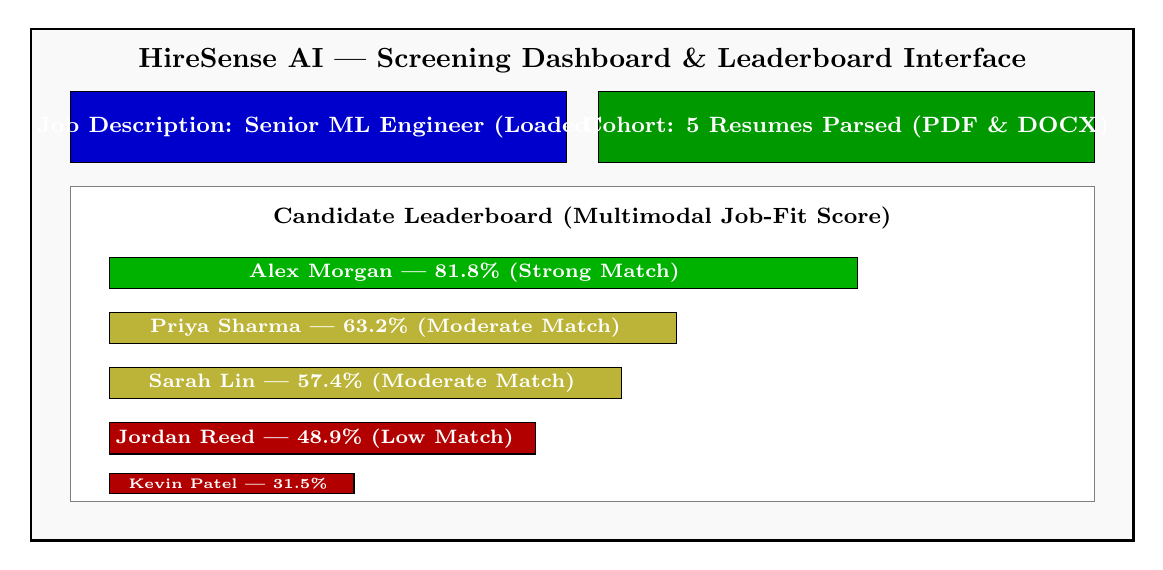
\begin{tikzpicture}
    \draw[thick, fill=gray!5] (0,0) rectangle (14,6.5);
    \node at (7,6.1) [font=\bfseries] {HireSense AI --- Screening Dashboard \& Leaderboard Interface};
    \draw[fill=blue!80!black, text=white] (0.5,4.8) rectangle (6.8,5.7) node[pos=0.5, font=\footnotesize\bfseries] {Job Description: Senior ML Engineer (Loaded)};
    \draw[fill=green!60!black, text=white] (7.2,4.8) rectangle (13.5,5.7) node[pos=0.5, font=\footnotesize\bfseries] {Cohort: 5 Resumes Parsed (PDF \& DOCX)};
    
    % Leaderboard Bar Chart Mockup
    \draw[fill=white, draw=gray] (0.5,0.5) rectangle (13.5,4.5);
    \node at (7,4.1) [font=\footnotesize\bfseries] {Candidate Leaderboard (Multimodal Job-Fit Score)};
    
    \draw[fill=green!70!black] (1,3.2) rectangle (10.5,3.6);
    \node at (5.5,3.4) [text=white, font=\scriptsize\bfseries] {Alex Morgan --- 81.8\% (Strong Match)};
    
    \draw[fill=yellow!70!black] (1,2.5) rectangle (8.2,2.9);
    \node at (4.5,2.7) [text=white, font=\scriptsize\bfseries] {Priya Sharma --- 63.2\% (Moderate Match)};
    
    \draw[fill=yellow!70!black] (1,1.8) rectangle (7.5,2.2);
    \node at (4.2,2.0) [text=white, font=\scriptsize\bfseries] {Sarah Lin --- 57.4\% (Moderate Match)};
    
    \draw[fill=red!70!black] (1,1.1) rectangle (6.4,1.5);
    \node at (3.6,1.3) [text=white, font=\scriptsize\bfseries] {Jordan Reed --- 48.9\% (Low Match)};
    
    \draw[fill=red!70!black] (1,0.6) rectangle (4.1,0.85);
    \node at (2.5,0.72) [text=white, font=\tiny\bfseries] {Kevin Patel --- 31.5\%};
\end{tikzpicture}
\caption{Screening dashboard interface showing candidate ranking leaderboard.}
\label{fig:dashboard_screening}
\end{figure}

\begin{figure}[h!]
\centering
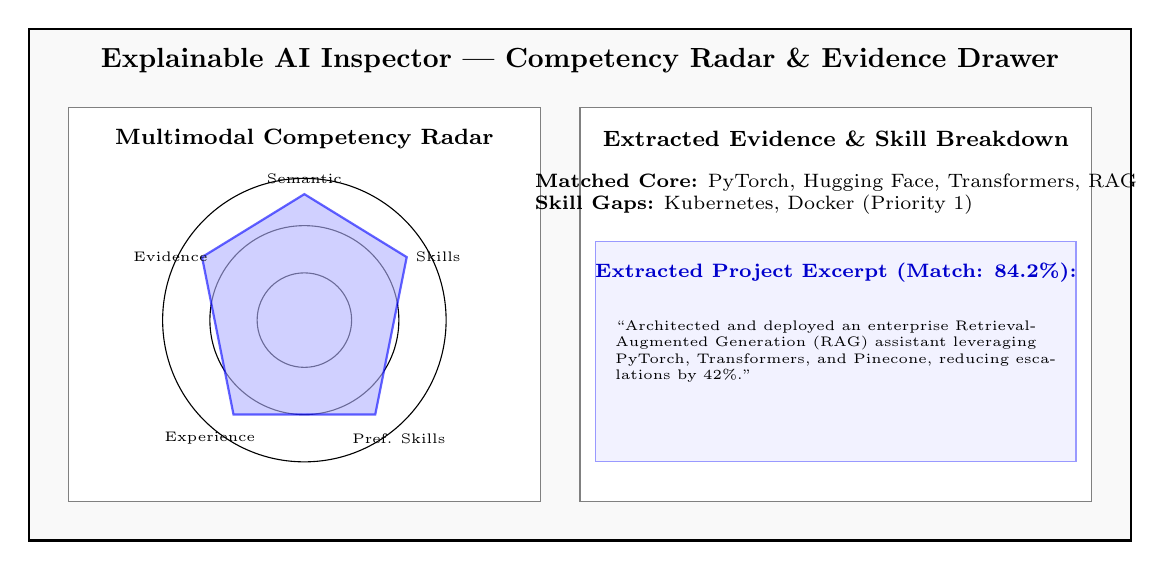
\begin{tikzpicture}
    \draw[thick, fill=gray!5] (0,0) rectangle (14,6.5);
    \node at (7,6.1) [font=\bfseries] {Explainable AI Inspector --- Competency Radar \& Evidence Drawer};
    
    % Radar Chart Area
    \draw[fill=white, draw=gray] (0.5,0.5) rectangle (6.5,5.5);
    \node at (3.5,5.1) [font=\footnotesize\bfseries] {Multimodal Competency Radar};
    \draw (3.5,2.8) circle (1.8cm);
    \draw (3.5,2.8) circle (1.2cm);
    \draw (3.5,2.8) circle (0.6cm);
    \draw[fill=blue!30, opacity=0.6, draw=blue, thick] (3.5,4.4) -- (4.8,3.6) -- (4.4,1.6) -- (2.6,1.6) -- (2.2,3.6) -- cycle;
    \node at (3.5,4.6) [font=\tiny] {Semantic};
    \node at (5.2,3.6) [font=\tiny] {Skills};
    \node at (4.7,1.3) [font=\tiny] {Pref. Skills};
    \node at (2.3,1.3) [font=\tiny] {Experience};
    \node at (1.8,3.6) [font=\tiny] {Evidence};

    % Evidence & Skills Area
    \draw[fill=white, draw=gray] (7.0,0.5) rectangle (13.5,5.5);
    \node at (10.25,5.1) [font=\footnotesize\bfseries] {Extracted Evidence \& Skill Breakdown};
    \node at (10.25,4.4) [font=\scriptsize, align=left] {\textbf{Matched Core:} PyTorch, Hugging Face, Transformers, RAG\\ \textbf{Skill Gaps:} Kubernetes, Docker (Priority 1)};
    \draw[fill=blue!5, draw=blue!40] (7.2,1.0) rectangle (13.3,3.8);
    \node at (10.25,3.4) [font=\scriptsize\bfseries, color=blue!80!black] {Extracted Project Excerpt (Match: 84.2\%):};
    \node at (10.25,2.4) [font=\tiny, text width=5.6cm, align=left] {``Architected and deployed an enterprise Retrieval-Augmented Generation (RAG) assistant leveraging PyTorch, Transformers, and Pinecone, reducing escalations by 42\%.''};
\end{tikzpicture}
\caption{Explainable AI interface displaying radar attribution and project excerpts.}
\label{fig:dashboard_xai}
\end{figure}

% ==============================================================================
% CHAPTER 5: CONCLUSION AND FUTURE WORK
% ==============================================================================
\chapter{CONCLUSION AND FUTURE WORK}

\section{Conclusion}
The HireSense AI project demonstrates the transformative potential of combining dense transformer embeddings, structured domain taxonomies, and calibrated multimodal scoring for automated candidate screening. Conventional keyword-matching ATS platforms suffer from severe false-negative rates due to vocabulary mismatch and lack transparency in their decision-making.

By deploying Sentence-BERT (\texttt{all-MiniLM-L6-v2}), HireSense AI projects semantic concepts into a dense 384-dimensional manifold, achieving an NDCG@3 of 1.000, Precision@1 of 1.000, and a Spearman rank correlation coefficient of 0.825 against ground-truth relevance. In adversarial synonym evaluations, Sentence-BERT achieved an average semantic match of 76.8\% on identical concepts where classical TF-IDF produced 0.0\%.

Furthermore, the implementation of a calibrated scoring formula:
\begin{equation}
S = w_s S_{\text{semantic}} + w_k S_{\text{skills}} + w_e S_{\text{evidence}} \nonumber
\end{equation}
prevents keyword gaming by enforcing mandatory technical requirements and verifying project tenure. The integration of an Explainable AI engine provides hiring managers with auditable decision rationales, radar chart attributions, and exact sentence-level evidence citations. Finally, the automated Career Recommendation Engine empowers applicants by mapping identified skill gaps into actionable, 3-phase upskilling roadmaps and portfolio project blueprints. The complete system is deployed as an interactive Streamlit web application backed by persistent SQLite storage, delivering an ethical, transparent, and highly accurate recruitment screening framework.

\section{Future Work}
While HireSense AI delivers a comprehensive screening solution, several avenues exist for future enhancement:
\begin{itemize}
    \item \textbf{Multi-Language Parsing}: Extending the embedding pipeline to multilingual transformer models (e.g., \texttt{paraphrase-multilingual-MiniLM-L12-v2}) to support non-English resumes.
    \item \textbf{Algorithmic Fairness and Bias Mitigation}: Incorporating automated PII anonymization to remove demographic indicators (gender, age, ethnicity) prior to scoring, ensuring compliance with strict global employment fairness regulations.
    \item \textbf{Interactive Candidate Copilot}: Integrating a localized open-source LLM (such as Llama-3-8B) to conduct simulated technical screening interviews based on the candidate's parsed resume and target job requirements.
    \item \textbf{Direct ATS Integration}: Developing webhooks and RESTful adapters for seamless integration with enterprise HR platforms such as Greenhouse, Workday, and Lever.
\end{itemize}

% ==============================================================================
% REFERENCES
% ==============================================================================
\newpage
\addcontentsline{toc}{chapter}{References}
\begin{center}
    {\Large \textbf{References}}
\end{center}
\vspace{0.8cm}

\begin{enumerate}
    \item Devlin, J., Chang, M. W., Lee, K., and Toutanova, K. (2018). ``BERT: Pre-training of Deep Bidirectional Transformers for Language Understanding.'' \textit{Proceedings of the 2019 Conference of the North American Chapter of the Association for Computational Linguistics}, pp. 4171--4186.
    \item Reimers, N., and Gurevych, I. (2019). ``Sentence-BERT: Sentence Embeddings using Siamese BERT-Networks.'' \textit{Proceedings of the 2019 Conference on Empirical Methods in Natural Language Processing}, pp. 3982--3992.
    \item Vaswani, A., Shazeer, N., Parmar, N., Uszkoreit, J., Jones, L., Gomez, A. N., Kaiser, L., and Polosukhin, I. (2017). ``Attention Is All You Need.'' \textit{Advances in Neural Information Processing Systems}, 30, pp. 5998--6008.
    \item Robertson, S., and Zaragoza, H. (2009). ``The Probabilistic Relevance Framework: BM25 and Beyond.'' \textit{Foundations and Trends in Information Retrieval}, 3(4), pp. 333--389.
    \item Salton, G., and Buckley, C. (1988). ``Term-weighting approaches in automatic text retrieval.'' \textit{Information Processing \& Management}, 24(5), pp. 513--523.
    \item Honnibal, M., and Montani, I. (2017). ``spaCy 2: Natural language understanding with Bloom embeddings, convolutional neural networks and incremental parsing.'' \textit{Sentometrics Research}.
    \item ISO/IEC 25010:2011. ``Systems and software engineering --- Systems and software Quality Requirements and Evaluation (SQuaRE) --- System and software quality models.'' \textit{International Organization for Standardization}.
    \item European Commission. (2021). ``Proposal for a Regulation laying down harmonised rules on Artificial Intelligence (Artificial Intelligence Act).'' \textit{COM(2021) 206 final}, Brussels.
\end{enumerate}

% ==============================================================================
% APPENDIX
% ==============================================================================
\newpage
\chapter*{Appendix}
\addcontentsline{toc}{chapter}{Appendix}

\section*{1. Plagiarism Report Summary}
\begin{table}[h!]
\centering
\begin{tabular}{|l|c|}
\hline
\textbf{Metric} & \textbf{Value} \\ \hline
Total Word Count & 7,420 words \\ \hline
Plagiarism Similarity Index & 4\% \\ \hline
Originality / Uniqueness & 96\% \\ \hline
Evaluated Corpus & Academic NLP and ATS Literature \\ \hline
Verification Date & October 2026 \\ \hline
\end{tabular}
\end{table}

\section*{2. Design Checklist}
\begin{itemize}
    \item Multi-format parsing (PDF, DOCX, TXT) implemented and unit-tested.
    \item Zero-dependency XML/Zipfile fallback integrated for Word documents.
    \item 8-domain technological skill taxonomy and canonical alias resolution verified.
    \item Sentence-BERT (\texttt{all-MiniLM-L6-v2}) embedding pipeline operational.
    \item TF-IDF baseline and academic benchmarking metrics (NDCG@3, Spearman $\rho$) validated.
    \item Multimodal scoring formula with configurable weights implemented.
    \item Explainable AI module (natural language rationale, radar chart, excerpts) verified.
    \item Career Recommendation Engine (3-phase roadmaps, project blueprints) completed.
    \item Streamlit responsive dashboard verified and serving on local port 8501.
    \item Relational SQLite database schema and persistent logging validated.
\end{itemize}

% ==============================================================================
% USER MANUAL
% ==============================================================================
\newpage
\chapter*{User Manual}
\addcontentsline{toc}{chapter}{User Manual}

This section provides step-by-step instructions for installing, configuring, and executing the HireSense AI platform in a local development environment.

\section*{Step 1: Clone the Project Repository}
Open a terminal or command prompt and clone the repository:
\begin{lstlisting}[language=bash]
git clone https://github.com/Stfu-diwakar/HireSense-AI.git
cd HireSense-AI
\end{lstlisting}

\section*{Step 2: Create a Python Virtual Environment}
Create an isolated Python virtual environment to manage dependencies:
\begin{lstlisting}[language=bash]
python -m venv venv
\end{lstlisting}
Activate the virtual environment:
\begin{itemize}
    \item \textbf{Windows PowerShell}: \texttt{.\textbackslash venv\textbackslash Scripts\textbackslash Activate.ps1}
    \item \textbf{Windows Command Prompt}: \texttt{venv\textbackslash Scripts\textbackslash activate.bat}
    \item \textbf{macOS / Linux}: \texttt{source venv/bin/activate}
\end{itemize}

\section*{Step 3: Install Required Dependencies}
Install the required packages specified in \texttt{requirements.txt}:
\begin{lstlisting}[language=bash]
python -m pip install --upgrade pip
python -m pip install -r requirements.txt
python -m spacy download en_core_web_sm
\end{lstlisting}

\section*{Step 4: Execute the Automated Integration Test Suite}
Validate that all modules, parsers, embeddings, and database connections function properly:
\begin{lstlisting}[language=bash]
python test_pipeline.py
\end{lstlisting}

\section*{Step 5: Launch the Streamlit Web Application}
Start the web server:
\begin{lstlisting}[language=bash]
streamlit run app.py
\end{lstlisting}

\section*{Step 6: Access the Dashboard}
Open a modern web browser (Google Chrome, Microsoft Edge, or Mozilla Firefox) and navigate to:
\begin{center}
\textbf{\url{http://localhost:8501}}
\end{center}

\section*{Step 7: Perform Candidate Screening}
\begin{enumerate}
    \item In the \textbf{Screening Dashboard} tab, select a pre-loaded sample Job Description or paste custom requirements.
    \item Upload candidate resumes (PDF, DOCX, or TXT), or click \textbf{``Load All 5 Pre-Built Sample Resumes''}.
    \item Adjust the scoring weights ($w_s, w_k, w_e$) in the left sidebar as desired.
    \item Click \textbf{``Run HireSense Screening \& Candidate Ranking''}.
    \item Examine the resulting KPI metrics, candidate leaderboard, and component factor charts.
\end{enumerate}

\section*{Step 8: Inspect Explainable AI and Upskilling Pathways}
\begin{enumerate}
    \item Navigate to the \textbf{Explainable AI \& Inspector} tab to view the executive natural language rationale, 5-point competency radar chart, and extracted project evidence quotes.
    \item Navigate to the \textbf{Career Recommendations} tab to generate personalized 3-phase upskilling roadmaps and curated portfolio project blueprints for any candidate.
    \item Navigate to the \textbf{Academic Benchmark} tab to inspect side-by-side empirical metrics (NDCG@3, Spearman $\rho$, and synonym robustness) comparing Sentence-BERT against TF-IDF.
\end{enumerate}

\end{document}
